\section{Matrix representations of networks}
\label{sec:ch4:mtx-rep}

A network itself lives in network space, which is the set of all possible networks. Network space is kind of abstract and inconvenient if we want to use traditional mathematics, so we'd generally like to represent networks with groups of numbers to make everything more concrete.

We generally represent networks with matrices. In addition to being computationally convenient, using matrices to represent networks lets us bring in a tools from linear algebra and statistics. Programmatically, using matrices also lets us use common \texttt{python} tools for array manipulation like \texttt{numpy}.

In \ref{alg:ch2} we used a common matrix representation of a network called the Adjacency Matrix. We will begin with that.

After that, we will explore the atom and then twin of the adjacency matrix: the degree matrix and the Laplacian matrix. We'll explore different types of Laplacians before moving on.

\subsection{Adjacency Matrices}

Adjacency matrices \cite{Godsil} are the beating heart of matrix representations of networks, and are the representation we will see the most throughout this book. Most other matrix representations that we see can either be derived from adjacency matrices, or are isomorphic to them. They work as follows: Let's say we have a network with $n$ nodes. We give each node an index (usually some value between $1$ and $n$, with one value per node) and then we create an $n \times n$ matrix. If there is an edge between node $i$ and node $j$, we fill the $(i, j)^{th}$ and $(j, i)^{th}$ values of the matrix with an entry, usually $1$ if our network has unweighted edges. In the case of undirected networks, we end up with a symmetric matrix with full of $1$s and $0$s, which completely represents the topology of our network.

The adjacency matrix looks like this:

\begin{align*}
    A &= \begin{bmatrix}
        a_{11} & ... & a_{1n} \\
        \vdots & \ddots & \vdots \\
        a_{n1} & ... & a_{nn}
    \end{bmatrix},
\end{align*}

Let's see this in action. We'll make a small, simple network with only three nodes, and then we'll see what it looks like as an adjacency matrix. To visualize this network, we'll use a layout plot, provided by \texttt{nx.draw\_network()}.

\begin{lstlisting}[style=python]
import numpy as np
import networkx as nx

G = nx.DiGraph()
# add nodes to the network
G.add_node("1", pos=(1,1))
G.add_node("2", pos=(4,4))
G.add_node("3", pos=(4,2))
# add edges to the network
G.add_edge("1", "2")
G.add_edge("2", "1")
G.add_edge("1", "3")
G.add_edge("3", "1")

# the coordinates in space to use for plotting the nodes
# in the layout plot
pos = {'1': (0, 0), '2': (1, 0), '3': (.5, .5)}

nx.draw_networkx(G, with_labels=True, node_color="tab:purple", pos=pos,
                font_size=10, font_color="whitesmoke", arrows=False, edge_color="black",
                width=1)
\end{lstlisting}

The resulting plot of the network is shown in Figure \ref{fig:ch4:basic_mtxs}(A). Our network has three nodes, labeled $1$, $2$, and $3$. Each of these three nodes is either connected or not connected to each of the two other nodes. We'll make a square matrix $A$, with 3 rows and 3 columns, so that each node has its own row and column associated to it.

So, let's fill out the matrix. We start with the first row, which corresponds to the first node, and move along the columns. If there is an edge between the first node and the node whose index matches the current column, put a $1$ in the current location. If the two nodes aren't connected, add a $0$. When you're done with the first row, move on to the second. Keep going until the whole matrix is filled with $0$'s and $1$'s. 

Since the second and third nodes aren't connected, there is a $0$ in locations $a_{2, 1}$ and $a_{1, 2}$. There are also zeroes along the diagonals, since nodes don't have edges with themselves. Here we plotted the adjacency matrix using \texttt{heatmap()}; we won't always show this plot in the future. 

\begin{lstlisting}[style=python]
from graphbook_code import heatmap
import matplotlib.pyplot as plt
import seaborn as sns

# convert the networkx graph to a numpy array
A = np.asarray(nx.to_numpy_matrix(G))

heatmap(A, annot=True, linewidths=.1, cbar=False, 
        title="Adjacency matrix", xticklabels=[1,2,3], xtitle="Node", 
        yticklabels=[1,2,3], ytitle="Node"
       )


\end{lstlisting}

The resulting adjacency matrix is shown in Figure \ref{fig:ch4:basic_mtxs}(B).

\begin{figure}[h]
    \centering
    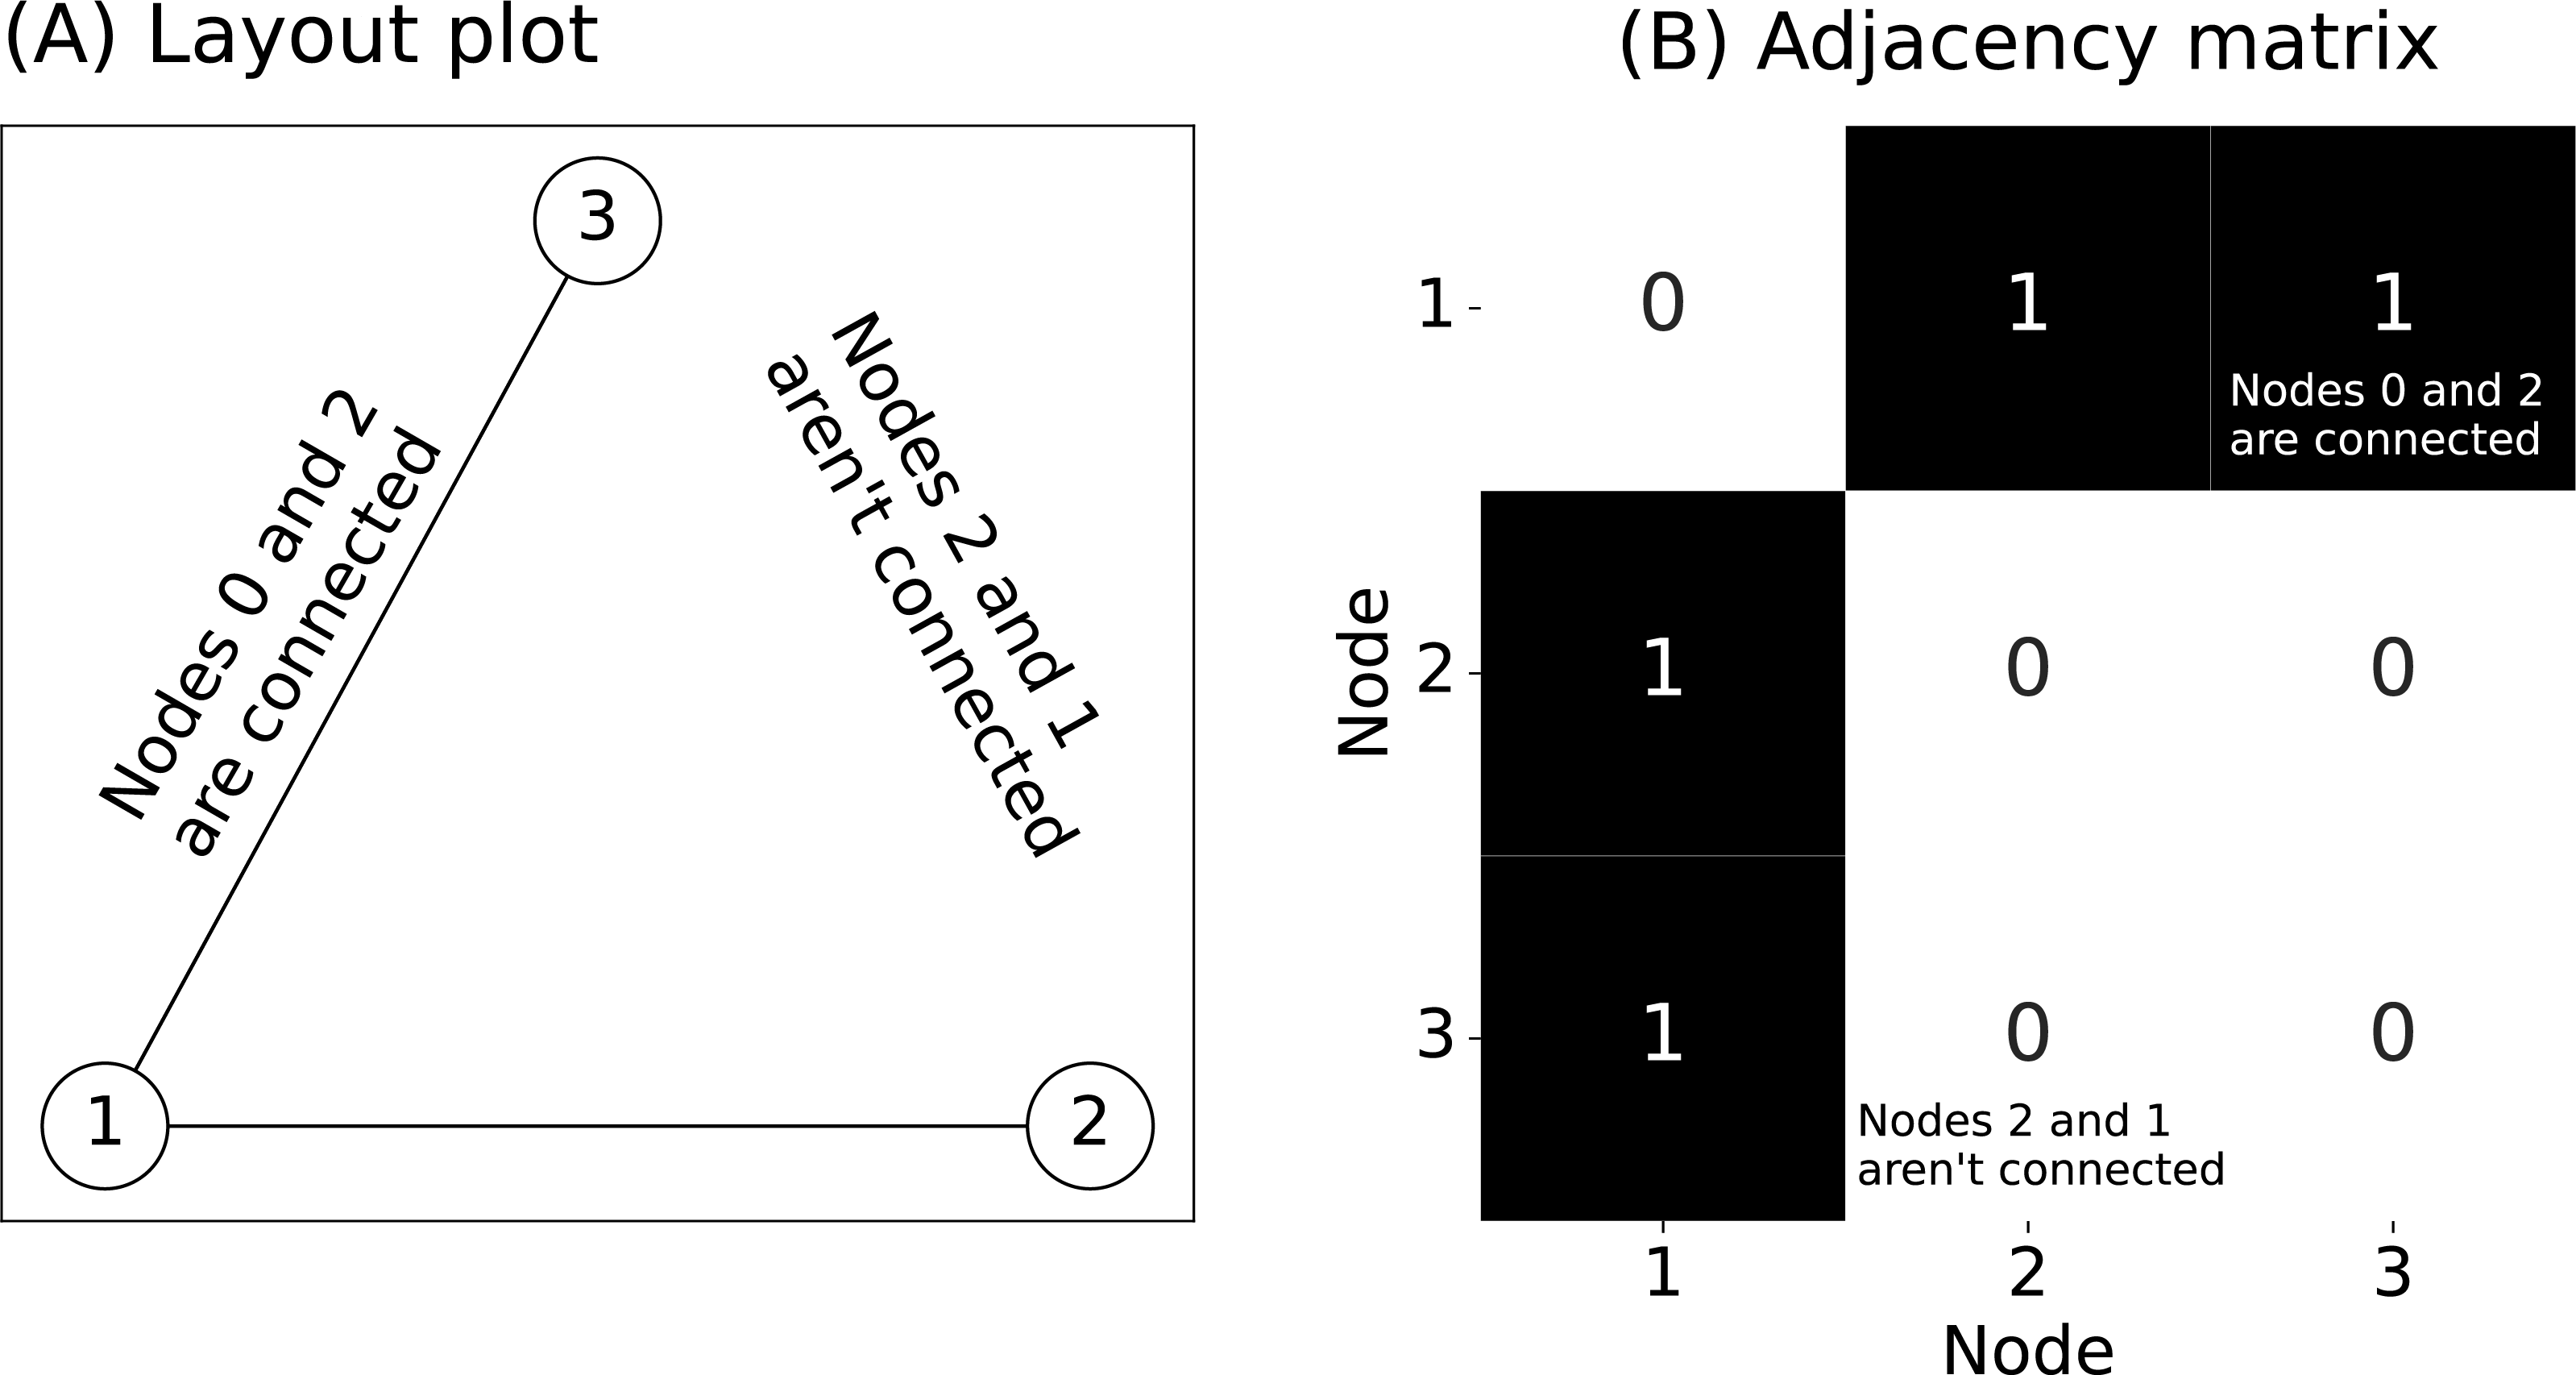
\includegraphics[width=0.8\linewidth]{representations/ch4/Images/basic_mtxs.png}
    \caption[Plotting a simple network as a layout plot and adjacency matrix heatmap]{\textbf{(A)} A layout plot of the network, where nodes are circles and edges are the lines connecting them. \textbf{(B)} the network, visualized as an adjacency matrix.}
    \label{fig:ch4:basic_mtxs}
\end{figure}

\subsection{The degree matrix}

Networks have a number of properties: edge count, number of nodes, average node connectivity, and so forth. The \emph{degree} of a node is one such property. It is simply the number of nodes that node is connected to.

The degree matrix takes this a step further, and acts to represent the degree of every node in the network. It doesn't completely describe our network, because we wouldn't be able to create an adjacency matrix just from a degree matrix -- we only know the number of connections, not which nodes are connected to each other. However, it pops up relatively often as a step in creating other matrices, so the degree matrix is useful to mention as its own entity. It is just a diagonal matrix with the values along the diagonal corresponding to the number of each edges each node has, also known as the \textit{degree} of each node. We'll learn more about the degree matrix in Section \ref{sec:ch4:prop-net}.

We can see the degree matrix for our network below. The diagonal element corresponding to node $1$ has the value of two, since it has two edges; the rest of the nodes have a value of $1$, since they each are only connected to the first node.

\begin{lstlisting}[style=python]
# Build the degree matrix D
degrees = np.count_nonzero(A, axis=0)
D = np.diag(degrees)
# plot it

heatmap(D, annot=True, linewidths=.1, cbar=False, 
        title="Degree matrix $D$", 
        xticklabels=[1,2,3], yticklabels=[1,2,3]
       ).set(xlabel="node", ylabel="node");

\end{lstlisting}
The degree matrix is shown in Figure \ref{fig:ch4:simple_lap}.

\subsection{The Laplacian Matrix}

The Laplacian Matrix is a direct derivative of the Adjacency Matrix. It is used in practice because it has a number of interesting mathematical properties which tend to be useful for analysis. For instance, the magnitude of its second-smallest eigenvalue, called the Fiedler eigenvalue, tells us how well-connected our network is -- the number of eigenvalues equal to zero is the number of connected components our network has (a concept you will be introduced to in Section \ref{sec:ch4:prop-net:lcc}). Incidentally, this means that the smallest eigenvalue of the Laplacian will always be 0, since any simple network always has at least one ``island''.

Another interesting property of the Laplacian is that the sum of its diagonals is twice the number of edges in the network. Because the sum of the diagonal matrix is the trace, and the trace is also equal to the sum of the eigenvalues, this means that the sum of the eigenvalues of the Laplacian is equal to twice the number of edges in the network.

The standard Laplacian Matrix $L$ \cite{Chung1996Dec} is just the adjacency matrix $A$ subtracted from the the degree matrix $D$:

\begin{align*}
 L = D - A
\end{align*}

Since the only nonzero values of the degree matrix is along its diagonals, and because the diagonals of an adjacency matrix never contain zeroes if its network doesn't have nodes connected to themselves, the diagonals of the Laplacian are just the degree of each node. The values on the non-diagonals work similarly to the adjacency matrix: they contain a $-1$ if there is an edge between the two nodes, and a $0$ if there is no edge.

The code below shows us what the Laplacian looks like. Since each node has exactly two edges, the degree matrix is just a diagonal matrix of all twos. The Laplacian looks like the degree matrix, but with -1's in all the locations where an edge exists between nodes $i$ and $j$. We can compute it using:

\begin{lstlisting}[style=python]
L = D - A
\end{lstlisting}

A plot of the Laplacian matrix as a heatmap, along with the degree and adjacency matrices, is shown in Figure \ref{fig:ch4:simple_lap}.
\begin{figure}[h]
    \centering
    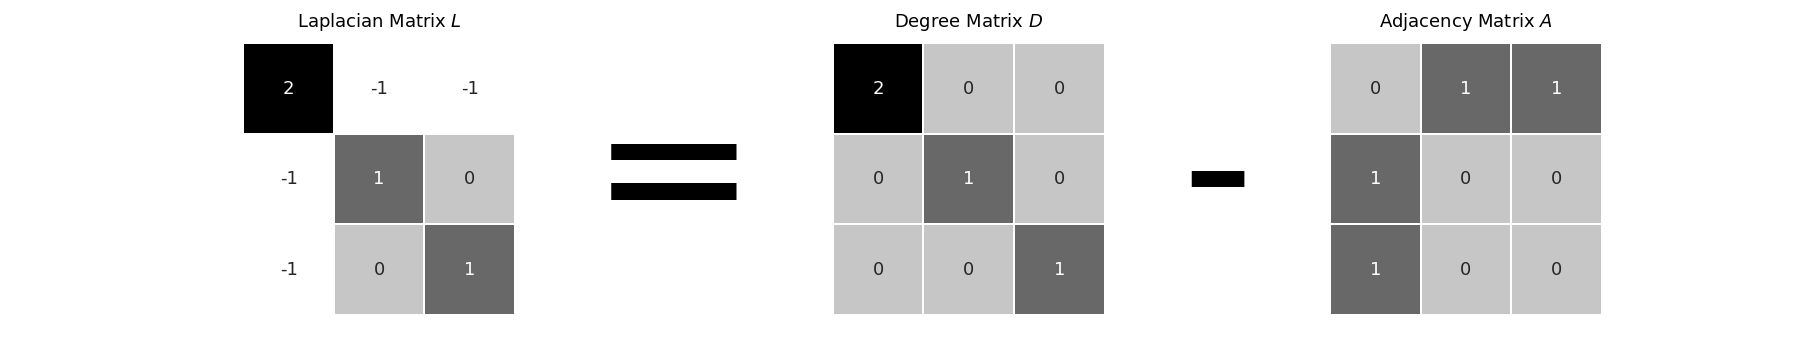
\includegraphics[width=\linewidth]{representations/ch4/Images/simple_lapl.png}
    \caption[Laplacian matrix]{The Laplacian matrix, along with the components that are used to compute it (the degree matrix and the adjacency matrix).}
    \label{fig:ch4:simple_lap}
\end{figure}

Laplacians and adjacency matrices will be used throughout this book. More details are in Chapter \ref{sec:ch6}.

\subsection{The Normalized Laplacian}
\label{sec:ch4:mat-rep:normlapl}

There are a few variations on the standard $D-A$ version of the Laplacian which are widely used in practice, and which (confusingly) are often also called the Laplacian. They tend to have similar properties. The Normalized Laplacian, $L^{norm.}$ is one such variation. The Normalized Laplacian \cite{Chung1996Dec} is defined as:

\begin{align*}
    L^{norm.} = D^{-1/2} L D^{-1/2} = I - D^{-1/2} A D^{-1/2}
\end{align*}

Where $I$ is the identity matrix (the square matrix with all zeroes except for ones along the diagonal). You can work through the algebra yourself if you'd like to verify that the second expression is the same as the third.

Below we can see the normalized Laplacian in code. We use \texttt{graspologic}'s \texttt{to\_laplacian()} function, with the \texttt{form} set to \texttt{I - DAD}, which computes $L^{norm.}$ above.
 
\begin{lstlisting}[style=python]
from graspologic.utils import to_laplacian
L_sym = to_laplacian(A, form="I-DAD")
\end{lstlisting}
A heatmap of the normalized Laplacian is shown in Figure \ref{fig:ch4:normlapl}(A).

We can understand the normalized Laplacian from the name: we can think of it as the Laplacian normalized by the degrees of the nodes associated with a given entry.

Here is what the operation is doing:

\begin{align*}
    L^{norm.} &= D^{-\frac{1}{2}}L D^{-\frac{1}{2}} \\
    &= \begin{bmatrix}
        d_{1} & & \\
        & \ddots & \\
        & & d_n
    \end{bmatrix}^{-\frac{1}{2}}\begin{bmatrix}
        l_{11} & ... & l_{1n} \\
        \vdots & \ddots & \vdots \\
        l_{n1} & ... & l_{nn}
    \end{bmatrix}
    \begin{bmatrix}
        d_{1} & & \\
        & \ddots & \\
        & & d_n
    \end{bmatrix}^{-\frac{1}{2}} \\
    &= 
    \begin{bmatrix}
        \frac{1}{\sqrt{d_1}} & & \\
        & \ddots & \\
        & & \frac{1}{\sqrt{d_n}}
    \end{bmatrix}\begin{bmatrix}
        l_{11} & ... & l_{1n} \\
        \vdots & \ddots & \vdots \\
        l_{n1} & ... & l_{nn}
    \end{bmatrix}
    \begin{bmatrix}
        \frac{1}{\sqrt{d_1}} & & \\
        & \ddots & \\
        & & \frac{1}{\sqrt{d_n}}
    \end{bmatrix} \\
    &= \begin{bmatrix}
        \frac{l_{11}}{d_1} & ... & \frac{l_{1n}}{\sqrt{d_1}\sqrt{d_n}} \\
        \vdots & \ddots & \vdots \\
        \frac{l_{n1}}{\sqrt{d_n}\sqrt{d_1}} & ... & \frac{l_{nn}}{d_n}
    \end{bmatrix}
\end{align*}
So the normalized laplacian has entries $l^{norm.}_{ij} = \frac{l_{ij}}{\sqrt{d_i}\sqrt{d_j}}$.

We can plug in the value of $L$ to obtain a similar relationship with the adjacency matrix $A$.
\begin{align*}
    L^{norm.} &=  D^{-\frac{1}{2}}L D^{-\frac{1}{2}} \\
    &=  D^{-\frac{1}{2}}(D - A) D^{-\frac{1}{2}} \\
    &= D^{-\frac{1}{2}}DD^{-\frac{1}{2}} - D^{-\frac{1}{2}}A D^{-\frac{1}{2}} \\
    &= D^{\frac{1}{2}}D^{-\frac{1}{2}} - D^{-\frac{1}{2}}A D^{-\frac{1}{2}} \\
    &= I_{n \times n} - D^{-\frac{1}{2}}A D^{-\frac{1}{2}}
\end{align*}

You could think of the $D^{-1/2} D D^{-1/2}$ term as spiritually the same as what we'd think of $\frac{D}{D}$ (if that were not undefined!), since it just works out to be the identity matrix. The $D^{-1/2} A D^{-1/2}$ is just doing the same thing to $A$ that we did to $L$. So we're normalizing the entries of the adjacency matrix by the degrees of the nodes a given entry is concerned with; that is, $\frac{a_{ij}}{\sqrt{d_i}\sqrt{d_j}}$.

One useful property of the normalized Laplacian is that its eigenvalues are bounded between 0 and 2, and so the Laplacian is a \emph{positive semi-definite matrix} (as are all matrices with exclusively positive or 0 eigenvalues). This means that a suite of linear algebra techniques, which may not run successfully on the adjacency matrix (which is \emph{not} positive semi-definite in its most raw form for simple networks, which we will learn about in the next chapter), can be executed on the network Laplacian. For more details about the properties of the Laplacian, check out \cite{Li2014Dec}.

\subsection{The \texttt{DAD} Laplacian}
\label{sec:ch4:mtx-rep:dad_laplacian}

In this book, a lot of what we will cover will be the \emph{spectral embedding} of the Laplacian (see Section \ref{sec:ch6:lse}). To understand the spectral embedding, we will need a related definition of a Laplacian, which we call the \texttt{DAD} Laplacian:

\begin{align*}
    L^{DAD} &= D^{-\frac{1}{2}}A D^{-\frac{1}{2}}
\end{align*}

$L^{DAD}$ and $L^{norm.}$ share some major similarities which are important to note here. Later in the book in Section \ref{sec:ch6:lse}, you will learn about the importance of the singular value decomposition for spectral embedding of Laplacians. Basically, what the singular value decomposition will allow us to do is look at the laplacian as a sum of much \emph{simpler} matrices. By ``simple'', what we mean here is that they can be represented as the product of two vectors. By looking only at the first few of these ``simple'' matrices, we can learn about the Laplacian and reduce a lot of noise in the Laplacian itself. The properties of looking at the \texttt{DAD} Laplacian are discussed at length in \cite{Chaudhuri2012Jun} and \cite{Amini2012Jul},

The most important connection is that these "simple" matrices will be \emph{identical} for $L^{norm.}$ and $L^{DAD}$, except for one important fact: they will be in \emph{reverse} order from one another. In $L^{norm}$, the matrices we will want to use will be the last few, and in $L^{DAD}$, the matrices we will want to use will be the first few. When we compute the singular value decomposition, there are ways to only compute the first few matrices without having to go through the trouble of computing \emph{all} of them, whereas the reverse is not true! To get the last few simple matrices, we would have to compute all of the preceding ones first. This means that to get the simple matrices we want, we can get much better computational performance using $L^{DAD}$ instead of $L^{norm}$.

We can compute the $L^{DAD}$ in \texttt{graspologic} similarly to above, but with \texttt{form="DAD"}:

\begin{lstlisting}[style=python]
L_dad = to_laplacian(A, form="DAD")
\end{lstlisting}

A heatmap of the \texttt{DAD} Laplacian is shown in Figure \ref{fig:ch4:normlapl}(B).

\subsection{The regularized Laplacian}
\label{ch4:mtx-rep:reg_laplacian}
The regularized Laplacian is an adaptation of the \texttt{DAD} Laplacian we learned about in the previous section. As it turns out, when networks have degree matrices where some of the degrees are really, really small, the \emph{spectral clustering} approach we will learn about in Section \ref{sec:ch7:comm_detect} is simply not going to perform very well. When we say it is not going to perform very well, what we mean is that the spectral clusterings are going to be extremely influenced by these nodes with really small node degrees. To overcome this hurdle, instead of using the \texttt{DAD} Laplacian, we can use the regularized Laplacian, defined extremely similarly to the \texttt{DAD} Laplacian, as:

\begin{align*}
    L^{rDAD}(\tau) &= D_\tau^{-\frac{1}{2}}A D_\tau^{-\frac{1}{2}}
\end{align*}

Where $\tau$ is a regularization constant which is greater than or equal to zero, and $D_\tau = D + \tau I$. When we put $\tau$ in parentheses here (that is, $(\tau)$), all that we mean is that $L^{rDAD}$ is a function of the particular regularization constant that we choose. Basically, what this is going to do is just "inflate" the diagonal elements of the degree matrix. So, if the degree for some of the nodes is extremely small, when we add a constant $\tau$ to them, we can increase the degrees by $\tau$. In effect, what this will do is make the nodes with really small degrees (which, like we said, might cause issues in the spectral clustering) a lot less impactful on the results that we obtain. Also, as we can see, if $\tau = 0$, then $L^{rDAD}(\tau) = L^{DAD}$. The regularized Laplacian is discussed at length in \cite{Qin2013Sep}.

Let's take a look at what $L^{rDAD}(\tau)$ and $L^{DAD}$ look like when we pick $\tau$ to be $1$. We can do this in \texttt{graspologic} using \texttt{form="R-DAD"}, and then setting \texttt{regularizer} appropriately:
\begin{lstlisting}[style=python]
tau = 1
L_rdad = to_laplacian(A, form="R-DAD", regularizer=tau)
\end{lstlisting}
The \texttt{R-DAD} Laplacian is shown in Figure \ref{fig:ch4:normlapl}(C).

We will learn about some other ways to handle nodes with very low degrees in Section \ref{sec:ch4:regularization} on Regularization.

\begin{figure}[h]
    \centering
    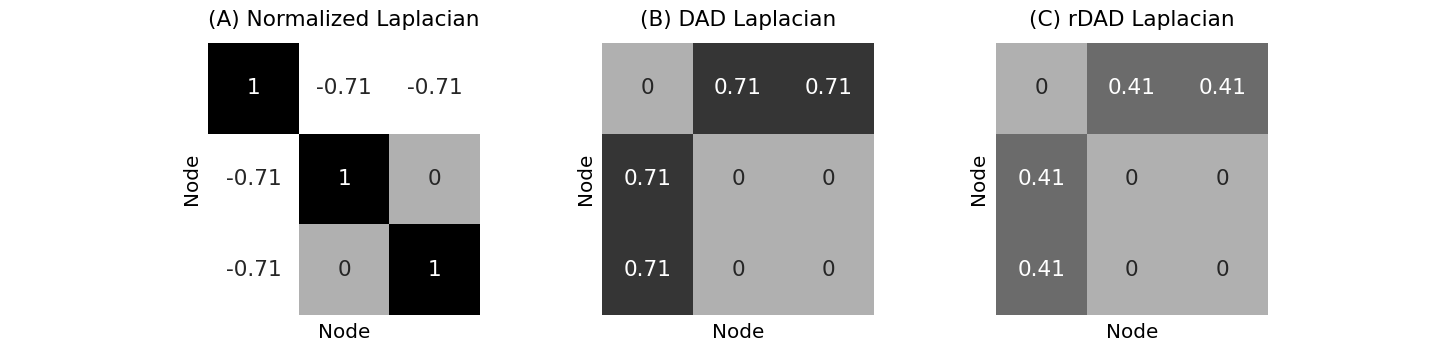
\includegraphics[width=\linewidth]{representations/ch4/Images/normlapls.png}
    \caption[comparison of normalized Laplacians]{Different variations of Laplacians for the same underlying network.}
    \label{fig:ch4:normlapl}
\end{figure}

\newpage